\subsection{Overview}

Text similarity measures play an increasingly important role in text related research and applications in tasks such as information retrieval, text classification, document clustering, topic detection, topic tracking, questions generation, question answering, essay scoring, short answer scoring, machine translation, text summarization and others. Finding similarity between words is a fundamental part of text similarity which is then used as a primary stage for sentence, paragraph and document similarities. There two way in which words can be similar each other, lexically if they share sequences of characters similar and  semantically if are used in the same context, used in the same way and so on. 

%%%%%%%%%%%%%%%%%%%%%%%%%%%%%%%%%%%%%%%%%%%%%%%%%%%%%%%%%%

\subsection{String-Based}

The world of lexical similarity con be divided in two categories: character-based and word-based.
To better understand what character-based means, here one of the most well known technique: Levenshtein distance.
\subsubsection{ Levenshtein distance}
 Levenshtein distance defines distance between two strings by counting the minimum number of operations needed to transform one string into the other, where an operation is defined as an insertion, deletion, or substitution of a single character, or a transposition of two adjacent characters.

This is an example:

\begin{itemize}
    \item kitten to sitten (substitution of "s" for "k").
    \item sitten to sittin (substitution of "i" for "e").
    \item sittin to sitting (insertion of "g" at the end).
\end{itemize}

Moving to the word-based,  the word or string similarity measures operate on string sequences and character composition. A string metric is a metric that measures similarity or dissimilarity (distance) between two text strings for approximate string matching or comparison.

\newpage
\subsubsection{Cosine Similarity}

Cosine similarity is a metric used to compute similarity between two objects using their feature vectors \cite{tversky1977features}. An object is characterized as a vector, and for a pair of vectors $\vec{\alpha}=(\alpha_{1},\alpha_{2},..,\alpha_{n})$ and $\vec{\beta}=(\beta_{1},\beta_{2},..,\beta_{n})$ there is an angle between them. Intuitively, the cosine similarity metric measures the similarity as the cosine of the corresponding angle between the two vectors and it is computed using the inner product as follows. 

\begin{equation} \label{eqn:Cosine}
CosineSim(\vec{\alpha},\vec{\beta}) = \frac{\sum_{i=1}^{n}\alpha_{i}\cdot \beta_{i}}{\sqrt{\sum_{i=1}^{n}(\alpha_{i})^{2} }\cdot \sqrt{\sum_{i=1}^{n}(\beta_{i})^{2}}}
\end{equation}

Figure \ref{fig:Cosine} illustrates the cosine similarity between two vectors $\vec{\alpha}$ and $\vec{\beta}$ in a three-dimension space. This can be thought as the similarity between two documents with three terms $t=(t_{1},t_{2},t_{3})$.

\begin{figure}[h!]
	\centering
	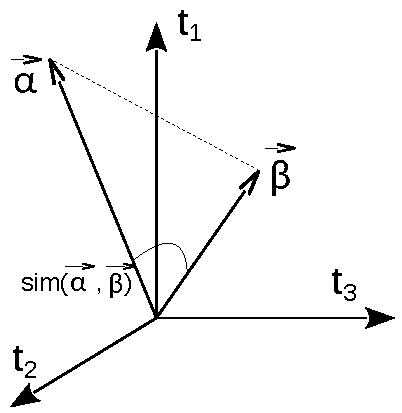
\includegraphics[width=0.25\textwidth]{images/Cosine.pdf}
	\caption{Cosine similarity between two feature vectors $\vec{\alpha}$ and $\vec{\beta}$}
	\label{fig:Cosine}
\end{figure}

Cosine similarity has been popularly adopted in many applications that are related to similarity measurement in various domains \cite{Huang:2012:LCD:2343876.2343884},\cite{Islam:2008:STS:1376815.1376819},\cite{Linden:2003:ARI:642462.642471},\cite{conf:iscis:MadylovaO09},\cite{Mihalcea:2006:CKM:1597538.1597662}. Among the similarity metrics being recalled in this deliverable, the prevalence of Cosine Similarity is obvious as it is utilized in almost all of them as follows: \textit{MUDABlue} \cite{10.1109/APSEC.2004.69}, \textit{CLAN} \cite{McMillan:2012:DSS:2337223.2337267}, \textit{CLANdroid} \cite{10.1109ICPC.2016.7503721}, \textit{LibRec} \cite{6671293}, \textit{SimApp} \cite{Chen:2015:SFD:2684822.2685305}, \textit{WuKong} \cite{Wang:2015:WSA:2771783.2771795}, \textit{TagSim} \cite{Lo:2012:DSA:2473496.2473616}, and \textit{RepoPal} \cite{10.1109/SANER.2017.7884605}.\\

This is an example of how the cosine similarity can be done  between two sentences.
These are the two string that we want to compare to see how much they are related each other.

\begin{itemize}
\item Julie loves me more than Linda loves me.
\item Jane likes me more than Julie loves me.
\end{itemize}
\newpage
From the strings is possible to count the occurrencies of each term, putting everything in a matrix.
\begin{figure}
	\begin{equation} \nonumber
	\bordermatrix{~ & string 1 & string 2 \cr	
		me 		& 2 & 2  \cr 
		Jane		& 0 & 1  \cr  
		Julia		& 1 & 1  \cr
		Linda 		& 1 & 0  \cr 
		likes		& 0 & 1  \cr
		loves		& 2 & 1  \cr
		more		& 1 & 1  \cr
		than		& 1 & 1  \cr	}
	\end{equation}
	\caption{The occurrencies.}
	\label{fig:TDM}
\end{figure}

Since in this kind of evaluation is not important the meaning or where the words are, is possibile to create the related vectore in order to compute the similarity.\\

	\begin{equation} \nonumber
	String1 = [2, 0, 1, 1, 0, 2, 1, 1]
	\end{equation}

	\begin{equation} \nonumber
	String2 = [2, 1, 1, 0, 1, 1, 1, 1]
	\end{equation}

Applying the cosine similarity formula this is the outcome:

\begin{equation} \label{eqn:Cosine}
CosineSim(\vec{\alpha},\vec{\beta}) = \frac{9}{\sqrt{12}\cdot \sqrt{10}} = 0.822
\end{equation}
This means that these strings are close each other 0.822, in a range bewteen 0.0 and 1.0.

%%%%%%%%%%%%%%%%%%%%%%%%%%%%%%%%%%%%%%%%%%%%%%%%%%%%%%%%%%  
\subsection{Corpus-Based}
\subsubsection{Term-Document Matrix}
 In Natural Language Processing \cite{Collobert:2011:NLP:1953048.2078186}, a term-document matrix (TDM) is used to represent the relationships between words and documents \cite{Turney:2010:FMV:1861751.1861756}. In a TDM, each row corresponds to a document and each column corresponds to a term. A cell in the TDM represents the weight of a term in a document. The most common weighting scheme used in document retrieval is the \emph{term frequency-inverse document frequency (tf-idf)} function \cite{Reed:2006:TNT:1193211.1193734}. If we consider a set of $n$ documents $D=(d_{1},d_{2},..,d_{n})$ and a set of terms $t=(t_{1},t_{2},..,t_{r})$ then the representation of a document $d \in D $ is vector $\vec{\delta}=(w_{1}^{d},w_{2}^{d},..,w_{r}^{d})$, where the weight $w_{k}^{d}$ of term $k$ in document $d$ is computed using the {\em tf-idf} function \cite{Ramos1999}:

\begin{equation} \label{tfidf} %\nonumber 
w_{k}^{d} =tf\cdot idf(k,d,D)= f_{k}^{d}\cdot log\frac{n}{\left | \left \{ d\in D: t_{k} \in d \right \} \right |} 
\end{equation}

where $f_{k}^{d}$ is the frequency of term $t_{k}$ in document $d$.

Another common weighting scheme uses only the frequency of terms in documents for cells in TDM, i.e. the number of occurrence of a term in a document, instead of {\em tf-idf}. As an example, we consider a set of three simple documents $D=(d_{1},d_{2},d_{3})$ as follows:

\begin{itemize}
	\item[+] $d_{1}$: \emph{She is nice.}
	\item[+] $d_{2}$: \emph{Today is nice.}
	\item[+] $d_{3}$: \emph{Nice is a nice city.}
\end{itemize}

\begin{figure}[h!]
	\begin{equation} \nonumber
	\bordermatrix{~ & she & is & today & a & nice & city \cr	
		d_{1} 		& 1 & 1 & 0 & 0 & 1 & 0 \cr 
		d_{2} 		& 0 & 1 & 1 & 0 & 1 & 0 \cr  
		d_{3} 		& 0 & 1 & 0 & 1 & 2 & 1 \cr }
	\end{equation}
	\caption{An example of a term-document matrix}
	\label{fig:TDM}
\end{figure}

The set of terms $t$ consists of $6$ elements, i.e. $t=(she$, $is$, $today$, $a$, $nice$, $city)$ and the corresponding term-document matrix for $D$ is depicted in Figure \ref{fig:TDM}.

TDM has been exploited to characterize software systems and finally to compute similarities between them \cite{10.1109/APSEC.2004.69},\cite{10.1109ICPC.2016.7503721},\cite{McMillan:2012:DSS:2337223.2337267}. In a TDM for software systems, each row represents a package, an API call or a function and each column represents a software system. A cell in the matrix is the number of occurrence of a package/an API/function in each corresponding software system. A TDM for software systems has a similar form to the matrix shown in Figure \ref{fig:TDM} where documents are replaced by software systems and terms are replaced by API calls.

\subsubsection{Latent Semantic Analysis}

The problem with the term-document matrix is that the intrinsic relationships among different terms of a document cannot fully be captured. Furthermore, same words can be used to explain different requirements or the other way around, the same requirements can be described using different words \cite{10.1109/APSEC.2004.69}. Latent Semantic Analysis (LSA), also known as Latent Semantic Indexing (LSI), has been proposed to overcome these problems \cite{Landauer1998}. The technique exploits a mathematical model that can infer latent semantic relationships to compute similarity. LSA represents the contextual usage meaning of words by statistical computations applied to a large corpus of text. It then generates a representation that captures the similarity of words and text passages. To perform LSA on a text, a term-document matrix is created to characterize the text. Afterwards, Singular Value Decomposition (SVD) - a matrix decomposition technique - is used in combination with LSA to reduce matrix dimensionality \cite{kb2005}. SVD takes a highly variable set of data entries as input and transforms to a lower dimensional space but reveals the substructure of the original data. Essentially, it decomposes a rectangular matrix into the product of three other matrices as given below\cite{kb2005}:

\begin{equation}
A_{mn}=U_{mm}S_{mn}V_{mn}^{T}
\end{equation}

in which

\begin{itemize}
	\item $U_{mm}$: Orthogonal matrix.
	\item $S_{mn}$: Diagonal matrix.
	\item $V_{mn}^{T}$: The transpose of an orthogonal matrix.
	\item $X$: Low Rank matrix.
\end{itemize}


$U_{mm}$ describes the original row entities as vectors of derived orthogonal factor values. $S_{mn}$ represents the original column entities in the same way, and $V_{mn}$ is a diagonal matrix containing scaling values. With the application of LSA it is possible to find the most relevant features and remove the least important ones by means of the reduced matrix $U_{mm}$. As a result, an equivalence of $A_{mm}$ can be constructed using the most relevant features. LSA helps reveal the latent relationship among words as well as among passages which cannot be guaranteed by a simple term-document matrix. The similarity measurement by LSA reflects adequately human perception of similarity and association among texts. Using LSA, similarities among documents are measured as the cosine of the angle between their row vectors (see Sec. \ref{sec:cosine}). LSA has been applied in \cite{10.1109/APSEC.2004.69},\cite{10.1109ICPC.2016.7503721},\cite{McMillan:2012:DSS:2337223.2337267} to compute similarities of software systems. The main disadvantage of LSA is that it is computational expensive when a large amount of information is analyzed.
Another very relevant issue related to LSA is the low rank approximation applied by the SVD procedure. If the singular values in $S_{mn}$ are ordered by size, the first k largest may be kept and the remaining smaller ones set to zero. The product of the resulting matrices is a matrix $X$ which is only approximately equal to $A_{mm}$ , and is of rank k . It can be shown that the new matrix $X$ is the matrix of rank k which is closest in the least squares sense to $A_{mm}$ .
The amount of dimension reduction, i.e., the choice of k , is critical to our work. Ideally, we want a value of k that is large enough to fit all the real structure in the data, but small enough so that we do not also fit the sampling error or unimportant details. The proper way to make such choices is an open issue in the factor analytic literature. In practice, we currently use an operational criterion - a
value of k which yields good retrieval performance. In our we decided a k value = numer of reposotories/2 [TO BE COMPLETED]
\newpage

An example.
Image that these are a set of document to be analyzed and we want to apply the procedure stated before.
\begin{itemize}
	\item doc1: Human machine interface for ABC computer applications
	\item doc2: A survey of user opinion of computer system response time
	\item doc3: The EPS user interface management system
	\item doc4: System and human system engineering testing of EPS
	\item doc5: Relation of user perceived response time to error measurement
	\item doc6: The generation of random, binary, ordered trees
	\item doc7: The intersection graph of paths in trees
	\item doc8: Graph minors IV: Widths of trees and well-quasi-ordering
	\item doc9: Graph minors: A survey
\end{itemize}

\begin{figure}[h!]
	\begin{equation} \nonumber
	\bordermatrix{~ & doc1 & doc2 & doc3 & doc4 & doc5 & doc6 & doc7 & doc8 & doc9 \cr	
		human	& 1 & 0 & 0 & 1 & 0 & 0 & 0 & 0 & 0 \cr
		interface	& 1 & 0 & 1 & 0 & 0 & 0 & 0 & 0 & 0 \cr
		computer	& 1 & 1 & 0 & 0 & 0 & 0 & 0 & 0 & 0 \cr    
		user 		& 0 & 1 & 1 & 0 & 2 & 0 & 0 & 0 & 0 \cr
		system 	& 0 & 1 & 1 & 2 & 0 & 0 & 0 & 0 & 0 \cr
		response	& 0 & 1 & 0 & 0 & 1 & 0 & 0 & 0 & 0 \cr
		time 		& 0 & 0 & 1 & 1 & 0 & 0 & 0 & 0 & 0 \cr
		EPS 		& 0 & 1 & 0 & 0 & 0 & 0 & 0 & 0 & 1 \cr
		survey	& 0 & 0 & 0 & 0 & 0 & 1 & 1 & 1 & 0 \cr
		trees 		& 0 & 0 & 0 & 0 & 0 & 0 & 1 & 1 & 1 \cr
		graph 		& 0 & 0 & 0 & 0 & 0 & 0 & 0 & 1 & 1 \cr
		minors		& 1 & 1 & 0 & 0 & 1 & 0 & 1 & 1 & 0 \cr	  }
	\end{equation}
	\caption{Term-Document matrix related to the example.}
	\label{fig:TDM}
\end{figure}

\begin{figure}[h!]
	\begin{equation} \nonumber
	\bordermatrix{ ~ \cr
		& 0.22 & -0.11 & 0.29 & -0.41 & -0.11 & -0.34 & 0.52 & -0.06 & -0.41 \cr
		& 0.20 & -0.07 & 0.14 & -0.55 & 0.28 & 0.50 & -0.07 & -0.01 & -0.11 \cr
		& 0.24 & 0.04 & -0.16 & -0.59 & -0.11 & -0.25 & -0.30 & 0.06 & 0.49 \cr
		& 0.40 & 0.06 & -0.34 & 0.10 & 0.33 & 0.38 & 0.00 & 0.00 & 0.01 \cr
		& 0.64 & -0.17 & 0.36 & 0.33 & -0.16 & -0.21 & -0.17 & 0.03 & 0.27 \cr
		& 0.27 & 0.11 & -0.43 & 0.07 & 0.08 & -0.17 & 0.28 & -0.02 & -0.05 \cr
		& 0.27 & 0.11 & -0.43 & 0.07 & 0.08 & -0.17 & 0.28 & -0.02 & -0.05 \cr
		& 0.30 & -0.14 & 0.33 & 0.19 & 0.11 & 0.27 & 0.03 & -0.02 & -0.17 \cr
		& 0.21 & 0.27 & -0.18 & -0.03 & -0.54 & 0.08 & -0.47 & -0.04 & -0.58 \cr
		& 0.01 & 0.49 & 0.23 & 0.03 & 0.59 & -0.39 & -0.29 & 0.25 & -0.23 \cr
		& 0.04 & 0.62 & 0.22 & 0.00 & -0.07 & 0.11 & 0.16 & -0.68 & 0.23 \cr
		& 0.03 & 0.45 & 0.14 & -0.01 & -0.30 & 0.28 & 0.34 & 0.68 & 0.18 \cr	  }
	\end{equation}
	\caption{$U_{mm}$x}
	\label{fig:TDM}
\end{figure}

\begin{figure}[h!]
	\begin{equation} \nonumber
	\bordermatrix{~  \cr	
		& 3.34 & 0 & 0 & 0 & 0 & 0 & 0 & 0 & 0 \cr
		& 0 & 2.54 & 0 & 0 & 0 & 0 & 0 & 0 & 0 \cr
		& 0 & 0 & 2.35 & 0 & 0 & 0 & 0 & 0 & 0 \cr
		& 0 & 0 & 0 & 1.64 & 0 & 0 & 0 & 0 & 0 \cr
		& 0 & 0 & 0 & 0 & 1.50 & 0 & 0 & 0 & 0 \cr
		& 0 & 0 & 0 & 0 & 0 & 1.31 & 0 & 0 & 0 \cr
		& 0 & 0 & 0 & 0 & 0 & 0 & 0.85 & 0 & 0 \cr
		& 0 & 0 & 0 & 0 & 0 & 0 & 0 & 0.56 & 0 \cr
		& 0 & 0 & 0 & 0 & 0 & 0 & 0 & 0 & 0.36 \cr
	  }
	\end{equation}
	\caption{ $S_{mn}$}
	\label{fig:TDM}
\end{figure}

\begin{figure}[h!]
	\begin{equation} \nonumber
	\bordermatrix{~  \cr	
		& 0.20 & 0.61 & 0.46 & 0.54 & 0.28 & 0.00 & 0.01 & 0.02 & 0.08 \cr
		& -0.06 & 0.17 & -0.13 & -0.23 & 0.11 & 0.19 & 0.44 & 0.62 & 0.53 \cr
		& 0.11 & -0.50 & 0.21 & 0.57 & -0.51 & 0.10 & 0.19 & 0.25 & 0.08 \cr
		& -0.95 & -0.03 & 0.04 & 0.27 & 0.15 & 0.02 & 0.02 & 0.01 & -0.03 \cr
		& 0.05 & -0.21 & 0.38 & -0.21 & 0.33 & 0.39 & 0.35 & 0.15 & -0.60 \cr
		& -0.08 & -0.26 & 0.72 & -0.37 & 0.03 & -0.30 & -0.21 & 0.00 & 0.36 \cr
		& 0.18 & -0.43 & -0.24 & 0.26 & 0.67 & -0.34 & -0.15 & 0.25 & 0.04 \cr
		& -0.01 & 0.05 & 0.01 & -0.02 & -0.06 & 0.45 & -0.76 & 0.45 & -0.07 \cr
		& -0.06 & 0.24 & 0.02 & -0.08 & -0.26 & -0.62 & 0.02 & 0.52 & -0.45 \cr	 
 }
	\end{equation}
	\caption{$V_{mn}^{T}$}
	\label{fig:TDM}
\end{figure}
The following image depict the result of the decomposition with a rank of 2.
\begin{figure}[h!]
	\begin{equation} \nonumber
	\bordermatrix{~ & doc1 & doc2 & doc3 & doc4 & doc5 & doc6 & doc7 & doc8 & doc9 \cr	
		human 	& 0.16 & 0.40 & 0.38 & 0.47 & 0.18 & -0.05 & -0.12 & -0.16 & -0.09 \cr
		interface 	& 0.14 & 0.37 & 0.33 & 0.40 & 0.16 & -0.03 & -0.07 & -0.10 & -0.04 \cr
		computer	& 0.15 & 0.51 & 0.36 & 0.41 & 0.24 & 0.02 & 0.06 & 0.09 & 0.12 \cr
		user 		& 0.26 & 0.84 & 0.61 & 0.70 & 0.39 & 0.03 & 0.08 & 0.12 & 0.19 \cr
		system 	& 0.45 & 1.23 & 1.05 & 1.27 & 0.56 & -0.07 & -0.15 & -0.21 & -0.05 \cr
		response 	& 0.16 & 0.58 & 0.38 & 0.42 & 0.28 & 0.06 & 0.13 & 0.19 & 0.22 \cr
		time 		& 0.16 & 0.58 & 0.38 & 0.42 & 0.28 & 0.06 & 0.13 & 0.19 & 0.22 \cr
		EPS 	 	& 0.22 & 0.55 & 0.51 & 0.63 & 0.24 & -0.07 & -0.14 & -0.20 & -0.11 \cr 
		survey 	& 0.10 & 0.53 & 0.23 & 0.21 & 0.27 & 0.14 & 0.31 & 0.44 & 0.42 \cr
		trees 		& -0.06 & 0.23 & -0.14 & -0.27 & 0.14 & 0.24 & 0.55 & 0.77 & 0.66 \cr
		graph 		& -0.06 & 0.34 & -0.15 & -0.30 & 0.20 & 0.31 & 0.69 & 0.98 & 0.85 \cr
		minors 	& -0.04 & 0.25 & -0.10 & -0.21 & 0.15 & 0.22 & 0.50 & 0.71 & 0.62 \cr	  }
	\end{equation}
	\caption{Matrix decomposed.}
	\label{fig:TDM}
\end{figure}

%%%%%%%%%%%%%%%%%%%%%%%%%%%%%%%%%%%%%%%%%%%%%%%%%%%%%%%%%%  
\subsection{Knowledge-Based}